\documentclass[border=5pt]{standalone}
\usepackage{tikz}
\usepackage{amssymb} % Para o símbolo \emptyset

\begin{document}
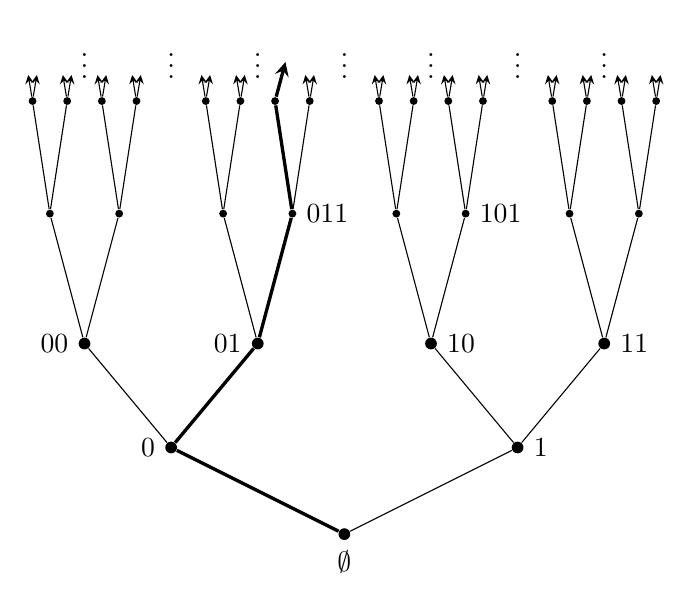
\begin{tikzpicture}[
    scale=1.1,
    dot/.style={circle, fill=black, inner sep=1.5pt},
    small dot/.style={circle, fill=black, inner sep=1.0pt},
    >=stealth
]

% Nível 0 (Raiz)
\node[dot, label=below:{$\emptyset$}] (root) at (0,0) {};

% Nível 1
\node[dot, label=left:{$0$}] (n0) at (-2,1) {};
\node[dot, label=right:{$1$}] (n1) at (2,1) {};

% Nível 2
\node[dot, label=left:{$00$}] (n00) at (-3,2.2) {};
\node[dot, label=left:{$01$}] (n01) at (-1,2.2) {};
\node[dot, label=right:{$10$}] (n10) at (1,2.2) {};
\node[dot, label=right:{$11$}] (n11) at (3,2.2) {};

% Nível 3
\node[small dot] (n000) at (-3.4,3.7) {};
\node[small dot] (n001) at (-2.6,3.7) {};
\node[small dot] (n010) at (-1.4,3.7) {};
\node[small dot, label=right:{$011$}] (n011) at (-0.6,3.7) {};
\node[small dot] (n100) at (0.6,3.7) {};
\node[small dot, label=right:{$101$}] (n101) at (1.4,3.7) {};
\node[small dot] (n110) at (2.6,3.7) {};
\node[small dot] (n111) at (3.4,3.7) {};

% Nível 4 (Folhas no topo)
\node[small dot] (l1)  at (-3.6,5) {};
\node[small dot] (l2)  at (-3.2,5) {};
\node[small dot] (l3)  at (-2.8,5) {};
\node[small dot] (l4)  at (-2.4,5) {};
\node[small dot] (l5)  at (-1.6,5) {};
\node[small dot] (l6)  at (-1.2,5) {};
\node[small dot, label=left:{}] (l7)  at (-0.8,5) {};
\node[small dot] (l8)  at (-0.4,5) {};
\node[small dot] (l9)  at (0.4,5) {};
\node[small dot] (l10) at (0.8,5) {};
\node[small dot] (l11) at (1.2,5) {};
\node[small dot] (l12) at (1.6,5) {};
\node[small dot] (l13) at (2.4,5) {};
\node[small dot] (l14) at (2.8,5) {};
\node[small dot] (l15) at (3.2,5) {};
\node[small dot] (l16) at (3.6,5) {};

% --- Arestas Padrão (linhas finas) ---
\draw (root) -- (n1);

\draw (n0) -- (n00);
\draw (n1) -- (n10);
\draw (n1) -- (n11);

\draw (n00) -- (n000);
\draw (n00) -- (n001);
\draw (n01) -- (n010);
\draw (n10) -- (n100);
\draw (n10) -- (n101);
\draw (n11) -- (n110);
\draw (n11) -- (n111);

\draw (n000) -- (l1);  \draw (n000) -- (l2);
\draw (n001) -- (l3);  \draw (n001) -- (l4);
\draw (n010) -- (l5);  \draw (n010) -- (l6);
\draw (n011) -- (l8);
\draw (n100) -- (l9);  \draw (n100) -- (l10);
\draw (n101) -- (l11); \draw (n101) -- (l12);
\draw (n110) -- (l13); \draw (n110) -- (l14);
\draw (n111) -- (l15); \draw (n111) -- (l16);

% --- Caminho em Destaque (linha grossa) ---
\draw[very thick] (root) -- (n0) -- (n01) -- (n011) -- (l7);
\draw[very thick, ->] (l7) -- (-0.68,5.45);

% --- Setas superiores das folhas ---
\draw[->] (l1) -- (-3.65,5.3);  \draw[->] (l1) -- (-3.55,5.3);
\draw[->] (l2) -- (-3.25,5.3);  \draw[->] (l2) -- (-3.15,5.3);
\draw[->] (l3) -- (-2.85,5.3);  \draw[->] (l3) -- (-2.75,5.3);
\draw[->] (l4) -- (-2.45,5.3);  \draw[->] (l4) -- (-2.35,5.3);
\draw[->] (l5) -- (-1.65,5.3);  \draw[->] (l5) -- (-1.55,5.3);
\draw[->] (l6) -- (-1.25,5.3);  \draw[->] (l6) -- (-1.15,5.3);
\draw[->] (l8) -- (-0.45,5.3);  \draw[->] (l8) -- (-0.35,5.3);
\draw[->] (l9) -- (0.35,5.3);   \draw[->] (l9) -- (0.45,5.3);
\draw[->] (l10) -- (0.75,5.3);  \draw[->] (l10) -- (0.85,5.3);
\draw[->] (l11) -- (1.15,5.3);  \draw[->] (l11) -- (1.25,5.3);
\draw[->] (l12) -- (1.55,5.3);  \draw[->] (l12) -- (1.65,5.3);
\draw[->] (l13) -- (2.35,5.3);  \draw[->] (l13) -- (2.45,5.3);
\draw[->] (l14) -- (2.75,5.3);  \draw[->] (l14) -- (2.85,5.3);
\draw[->] (l15) -- (3.15,5.3);  \draw[->] (l15) -- (3.25,5.3);
\draw[->] (l16) -- (3.55,5.3);  \draw[->] (l16) -- (3.65,5.3);

% --- Pontos de continuação (reticências verticais) ---
\node at (-3.0, 5.5) {$\vdots$};
\node at (-2.0, 5.5) {$\vdots$};
\node at (-1.0, 5.5) {$\vdots$};
\node at (0.0, 5.5)  {$\vdots$};
\node at (1.0, 5.5)  {$\vdots$};
\node at (2.0, 5.5)  {$\vdots$};
\node at (3.0, 5.5)  {$\vdots$};

\end{tikzpicture}
\end{document}